%% Coherence sweet spots across superconducting qubit architectures
%%
%% VENUE: IEEE Transactions on Quantum Engineering (IEEEtran, journal mode).
%% Confirmed by the author. Journal mode rather than conference mode because the
%% paper runs to 8 pages, past the 6-page limit typical of IEEE conferences.
%%
%% Build:  tectonic -X compile main.tex     (or: latexmk -pdf main.tex)
%%
%% EVERY number in this paper is traceable to data/headline_provenance_ledger.csv,
%% which 05_summary.ipynb regenerates and asserts. If you change a number here,
%% change it there first and let the ledger verify it.
\documentclass[journal]{IEEEtran}
\usepackage{amsmath,amssymb,booktabs,graphicx,siunitx,url}
\usepackage[hidelinks]{hyperref}
\usepackage{xurl}   % break long URLs; without it the repo link forces badness-10000 lines

\begin{document}

\title{Coherence Sweet Spots Are Frequency Minima in Disguise:\\
Metric Sensitivity in Transmon and Fluxonium Design Spaces}

\author{Ishita~Bera%
\thanks{I. Bera is an independent researcher; this work was carried out as a
self-directed project without institutional or financial support.
E-mail: ishitabera4@gmail.com}%
\thanks{Code, data and figures:
\url{https://github.com/ishitabera/quantum-coherence-sweet-spots-transmon-fluxonium}}}

\maketitle

\begin{abstract}
That dielectric loss scales with transition frequency is well known, and it implies that a
lower-frequency qubit relaxes more slowly at fixed quality factor. We show that this has a
sharper consequence for design studies than is usually acknowledged: under a common noise
model, modelled $T_2$ over the transmon $(E_J, E_C)$ plane correlates with $f_{01}$ at
$r = -0.9999$ within the transmon regime, and over the fluxonium $(E_J, E_L)$ plane at
$-0.9973$. Each plane carries one effective degree of freedom, so a raw $T_2$ maximum locates
the lowest-frequency corner of the swept domain rather than a design, and both of our own
headline optima prove to be grid-edge points outside any usable frequency band. Controlling
for frequency changes the conclusions. The transmon has no interior optimum in $E_J/E_C$: at
fixed $f_{01}$, $T_2$ is flat to 4.8\% across a tenfold range while the anharmonicity falls
$7.3\times$, so charge insensitivity is bought with gate speed rather than coherence, and any
reported optimum sits on whichever regime threshold is imposed. The fluxonium does have a
genuine interior optimum, visible only once second-order $1/f$ flux dephasing is included, but
it lies at $10$--$75$\,MHz where $\bar n_{\rm th} = 4$--$32$. For the cross-architecture
question we find no single answer: the ratio spans ${\sim}700\times$ across defensible metrics,
and at matched frequency the $T_2$ advantage inverts to a median $0.86\times$ across the
literature noise band. A lab-frame pulse simulation settles the widest of those metrics at
$36$--$58\times$, excluding both analytic bounds, because the fluxonium's drive couples
$10.2\times$ more strongly to its leakage transition than to its qubit transition.
\end{abstract}

\begin{IEEEkeywords}
superconducting qubits, transmon, fluxonium, decoherence, $1/f$ noise, sweet spots
\end{IEEEkeywords}

\section{Introduction}

Superconducting qubit design is routinely discussed in terms of \emph{sweet spots}:
bias points at which the transition frequency is stationary with respect to a noise
coordinate, so that first-order dephasing vanishes. The transmon achieves this by
exponential suppression of charge dispersion~\cite{koch2007}; the fluxonium achieves it at
half a flux quantum, where $\partial\omega_{01}/\partial\Phi = 0$ by
symmetry~\cite{manucharyan2009,nguyen2019}. Both are then said to have a coherence sweet
spot in \emph{design} space as well, and the point of best modelled $T_2$ over a swept
parameter plane is reported as an optimum.

This paper argues that the second usage does not survive scrutiny, and that the error is
systematic rather than incidental. We address three questions:

\begin{itemize}
\item[\textbf{Q1}] Where are the coherence optima across the transmon $(E_J, E_C)$ and
      fluxonium $(E_J, E_C, E_L, \Phi)$ design spaces?
\item[\textbf{Q2}] Which noise channel dominates where?
\item[\textbf{Q3}] Does the fluxonium's flux sweet spot buy more robustness than the
      transmon's charge insensitivity, and at what cost?
\end{itemize}

Our central methodological claim is that Q1 and Q3 cannot be answered without controlling
for the transition frequency, and that once controlled the conventional answers change sign
or dissolve. Our central negative result is that the fluxonium's coherence advantage at
matched frequency does not survive the uncertainty in the noise amplitudes that the model
itself assumes.

Figure~\ref{fig:summary} summarises the study. All results are model-based estimates under
literature noise amplitudes. They are not predictions of device performance, and
Section~\ref{sec:calibration} quantifies how far they sit from measurement.

\begin{figure*}[t]
\centering
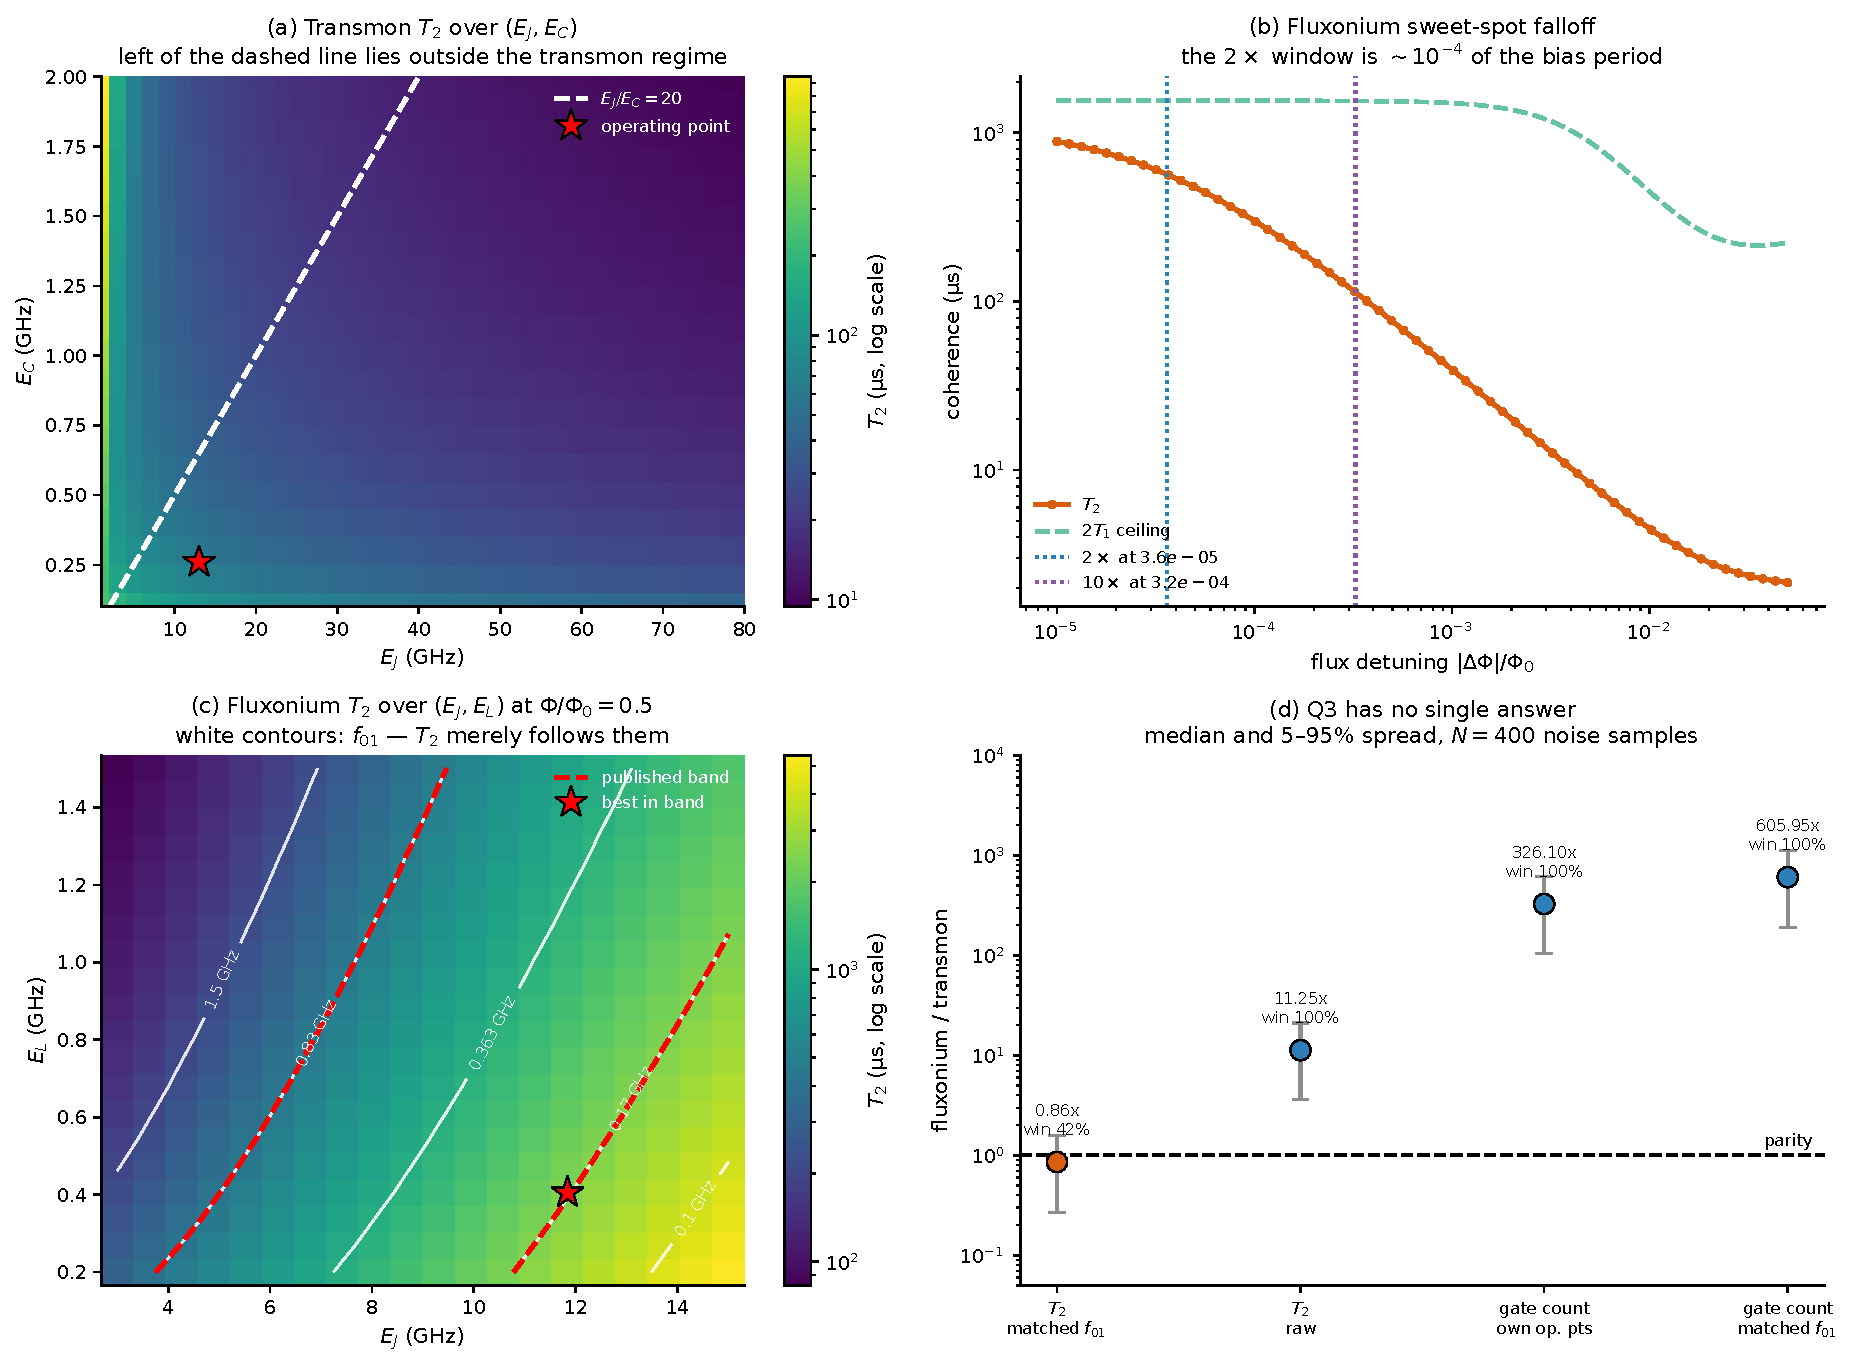
\includegraphics[width=\textwidth]{figures/summary_figure.pdf}
\caption{The study in four panels. (a) Transmon $T_2$ over $(E_J, E_C)$ at $n_g = 0$; left of
the dashed line is the charge-qubit regime, whose numbers are not transmon results. (b) The
fluxonium sweet-spot falloff on a log-detuning axis, with the $2T_1$ ceiling and the two-
and tenfold loss points; on a linear flux axis the entire collapse hides inside the first
0.1\% of the plot. (c) Fluxonium $T_2$ over $(E_J, E_L)$ at half flux, with $f_{01}$ contours
in white --- the $T_2$ structure merely follows them, which is the confound this paper is
about. (d) The Q3 answer under each metric, with the 5--95\% spread over $N=400$ noise-amplitude
draws; orange marks the metrics in which the fluxonium wins fewer than 90\% of samples.}
\label{fig:summary}
\end{figure*}

\section{Related Work and Contribution}

\subsection{What is already established}

The frequency scaling we build on is not new. Dielectric loss from two-level-system defects at
surfaces and interfaces is the dominant relaxation channel in transmons, with the relaxation
rate approximately proportional to the surface participation ratio~\cite{wang2015}; at fixed
quality factor the rate grows with $\omega_{01}$, so a lower-frequency qubit relaxes more
slowly. Design-space optimisation under noise models is likewise established: Papi\v{c}
\emph{et al.} identify optimal transmon parameter ranges through comprehensive noise modelling
including charge-parity effects~\cite{papic2024}, and Ram \emph{et al.} give a staged framework
spanning circuit design, spectral analysis and calibration for both
architectures~\cite{ram2025}. Experimentally, fluxonium coherence has advanced well past the
devices we calibrate against: Somoroff \emph{et al.} report $T_2 = 1.43$\,ms with average gate
fidelity $0.99991$~\cite{somoroff2023}.

Two works are close enough to this one to be worth locating precisely.

McRae \emph{et al.}~\cite{mcrae2021} argue that coherence metrics cannot currently be compared
across measurements, devices and laboratories, because temporal fluctuation, TLS dynamics and
unreported experimental detail dominate the differences being claimed. Their concern is
\emph{experimental} reproducibility. The present paper makes the modelling analogue of that
argument: a comparison drawn from a swept design space is equally unreliable unless the
control variable and the figure of merit are stated with the number.

Lange \emph{et al.}~\cite{lange2025} compare transmon and fluxonium lattices directly, and---
importantly---do so under an explicit control, designing each architecture for similar gate
speed and fidelity before comparing. Their figures of merit are residual $ZZ$ cross-talk and
state localisation; \emph{coherence is not among them}. Our work is complementary: same
instinct about controlled comparison, different quantity.

\subsection{Contribution}

Our contribution is not the frequency scaling but its consequence for how design studies are
read:

\begin{enumerate}
\item We quantify the confound as a near-complete rank deficiency of the design plane in
      \emph{both} architectures ($|r| > 0.99$), so that a raw $T_2$ optimum is a statement
      about where the sweep stopped rather than about a design.
\item We show the transmon optimum is pinned to whatever regime threshold is imposed, across
      eight thresholds spanning $E_J/E_C = 15$--$60$, so the threshold and not the
      optimisation is the substantive choice.
\item We show that including second-order $1/f$ flux dephasing creates an interior fluxonium
      optimum that a first-order model---the standard tooling default---does not see at all.
\item We show the architecture comparison spans two orders of magnitude across defensible
      metrics, and settle the widest of those metrics by direct pulse simulation.
\end{enumerate}

We are not aware of a study reporting the metric sensitivity of the transmon--fluxonium
coherence comparison explicitly. That statement rests on the survey above, which is not
exhaustive; the individual ingredients are all known, and the claim is about their combination.

\subsection{A caveat on our own control}

Matching $f_{01}$ removes the dominant confound but not all of it. Dielectric loss also depends
on geometry and surface participation, which differ between architectures and which a
Hamiltonian-level model does not capture~\cite{wang2015}, and real devices fluctuate in ways
no static model represents~\cite{mcrae2021}. Frequency matching is necessary, not sufficient,
and our matched-frequency numbers should be read as removing one large confound rather than
as a fully controlled experiment.

\section{Model and Conventions}

\subsection{Noise channels}

Coherence is estimated with \texttt{scqubits}~\cite{groszkowski2021}. Rates add,
\begin{equation}
\frac{1}{T_2} = \frac{1}{2T_1} + \sum_k \frac{1}{T_{\phi,k}},
\label{eq:rates}
\end{equation}
and channels are selected per architecture. A plain transmon has no flux loop, so
$1/f$ flux dephasing is not a supported channel for it; the fluxonium has no charge
dispersion to speak of. Table~\ref{tab:channels} lists the assignment.

\begin{table}[t]
\caption{Noise channels by architecture.}
\label{tab:channels}
\centering
\small
\begin{tabular}{@{}llcc@{}}
\toprule
Channel & \texttt{scqubits} method & Tmon & Flux\\
\midrule
Dielectric loss ($T_1$)   & \texttt{t1\_capacitive}          & \checkmark & \checkmark\\
Quasiparticle ($T_1$)     & \texttt{t1\_quasipart...}        & --         & \checkmark\\
$1/f$ flux, 1st order     & \texttt{tphi\_1\_over\_f\_flux}  & --         & \checkmark\\
$1/f$ flux, 2nd order     & \emph{this work}                 & --         & \checkmark\\
Charge / offset           & \texttt{tphi\_1\_over\_f\_ng}    & \checkmark & --\\
Critical current          & \texttt{tphi\_1\_over\_f\_cc}    & \checkmark & \checkmark\\
\bottomrule
\end{tabular}
\end{table}

Noise amplitudes are $Q_{\rm cap} = 10^6$, $A_{n_g} = 10^{-4}$, $A_\Phi = 10^{-6}\,\Phi_0$,
$A_{cc} = 10^{-7}$; the flux amplitude sits at the optimistic end of the measured range, which
clusters near $1$--$2\,\mu\Phi_0$ across flux-sensitive devices~\cite{yan2016,nguyen2019}. Temperature, quasiparticle density and the $1/f$ cutoffs are the
\texttt{scqubits} defaults ($T = \SI{15}{\milli\kelvin}$, $x_{qp} = 3\times10^{-6}$,
$t_{\rm exp} = \SI{10}{\micro\second}$) and are recorded with every result, since they set
the answers and are easily left undeclared.

\subsection{Second-order flux dephasing}

\texttt{scqubits} implements $1/f$ dephasing to first order in
$\partial\omega_{01}/\partial\lambda$, which vanishes identically at a sweet spot; the
package returns a divergent time there, documented behaviour rather than a
bug~\cite{groszkowski2021}. The physical rate at half flux is second order, and we implement
the closed form used for fluxonium by Nguyen \emph{et al.}~\cite{nguyen2019}, after
Ithier \emph{et al.}~\cite{ithier2005}:
\begin{equation}
\Gamma_\Phi^{(2)} = \frac{\partial^2\omega_{01}}{\partial\Phi^2}\, A_\Phi^2 .
\label{eq:secondorder}
\end{equation}
Equation~\eqref{eq:secondorder} carries no logarithmic factor. Other treatments attach a
prefactor of order $|\ln(\omega_{\rm low}t_{\rm exp})|$ or its square, which moves the answer
by two orders of magnitude; we report the convention dependence rather than burying it. The
required curvature is Richardson-extrapolated, because a plain central difference is still
4\% from converged in the deep-well regime where this channel matters most.

\subsection{A declared modelling choice}

Passing $Q_{\rm cap}$ explicitly installs a \emph{flat}, frequency-independent quality factor
in place of the \texttt{scqubits} default $Q_{\rm cap}(\omega) \propto \omega^{-0.7}$
\cite{smith2020}. At the fluxonium sweet spot the two differ by $7.1\times$ in $T_1$, making
this the largest single modelling choice in the study. The spread is one-sided rather than
symmetric: Nguyen \emph{et al.} fit their own $T_1$-versus-frequency data with
$\tan\delta_C \propto \omega^{0.15}$, and at $f_{01} = \SI{0.363}{\giga\hertz}$ the flat
model sits $1.52\times$ from their measured exponent while the \texttt{scqubits} default sits
$4.7\times$ from it. We retain the flat value as both the conservative and the
better-supported choice, and declare it.

\section{Validation}
\label{sec:validation}

Forty-four checks establish the pipeline before any result is generated. They compare
against exact Hamiltonian symmetries (machine precision), basis-size convergence, analytic
limits from Koch \emph{et al.}, and---in seven cases---data measured on real devices.

The sharpest analytic anchor is Koch's worked charge-dephasing example: at
$E_J = \SI{30}{\giga\hertz}$, $E_C = \SI{0.35}{\giga\hertz}$ and $A = 10^{-4}$ he quotes
$T_2 \sim \SI{8}{\second}$; feeding our computed charge dispersion through his Eq.~(5.9)
gives \SI{8.75}{\second}. The maximum charge-dispersion derivative reproduces his
$1.5\times10^{-4}E_C$ at $E_J/E_C = 50$ to a ratio of $0.830$, the expected sign for an
asymptotic expression approached from below.

Against Manucharyan \emph{et al.}~\cite{manucharyan2009}, the lowest two transitions at
$\Phi_{\rm ext} = 0$ are reproduced to better than 0.7\% under \emph{every} one of that
paper's three published parameter sets, and a single four-parameter fit reproduces all six
digitized lines across two flux biases to an RMS of \SI{0.0102}{\giga\hertz}. We note that
those three parameter sets---the rounded main-text values and two Table~I least-squares
fits---span 9.5\% in $f_{01}$ at the flux sweet spot, so agreement quoted against the
main-text values alone overstates the constraint.

The third transition at $\Phi_{\rm ext} = 0$ is excluded from this claim for a physical
reason rather than a loose tolerance. Its bare value lies within \SIrange{0.14}{0.36}{\giga\hertz}
of the junction-array mode that Manucharyan's extended model places at
\SI{10.78}{\giga\hertz}, with a $0$--$3$ coupling near \SI{0.53}{\giga\hertz}: the coupling
exceeds the detuning by $1.5$--$3.7\times$, so the line is strongly hybridized and no
bare-circuit model can reproduce it. Explicit diagonalization of the fluxonium coupled to
both array modes confirms that this is a $\Phi_{\rm ext} = 0$ effect and bounds what our
ideal-superinductance model gives up by omitting them: the dressed $f_{01}$ shifts by $-16\%$
at $\Phi_{\rm ext} = 0$ but by only $-0.43\%$ at the flux sweet spot, where every coherence
number in this study is evaluated---smaller than the 9.5\% spread across the paper's own
published parameter sets.

Finally, the second-order channel of Eq.~\eqref{eq:secondorder} is the one piece of physics
implemented here rather than taken from established tooling, so it is validated against a
published number rather than against its own formula. Evaluated on Nguyen's nine devices at
their measured $A_\Phi = 1.8\,\mu\Phi_0$ it yields $T_\phi^{(2)} = 15$--\SI{804}{\milli\second},
clearing their stated bound of $>\SI{10}{\milli\second}$ for all qubits on every device.

\section{The Transmon Design Plane}

We sweep $E_J \in [1, 80]$, $E_C \in [0.1, 2.0]$\,GHz at $n_g = 0$ and $n_g = 0.25$
(800 points each), and refine to a $65\times53$ grid over $E_J \in [4,20]$,
$E_C \in [0.08, 0.6]$\,GHz.

\subsection{The confound}

Within the transmon regime $E_J/E_C \ge 20$, $\mathrm{corr}(\log T_2, \log f_{01}) = -0.9999$.
The plane contains one degree of freedom, not two. The reason is structural rather than
numerical: dielectric loss dominates $T_1$ everywhere in the regime, with
$\Gamma \propto |\langle 0|\hat n|1\rangle|^2 S(\omega_{01})$. Since
$|\langle 0|\hat n|1\rangle|^2 \propto \sqrt{E_J/E_C}$ and $S \propto E_C$, the rate goes as
$\sqrt{E_JE_C} \propto \omega_{01}$---a function of frequency alone. Consequently the best
$T_2$ point of the swept plane, \SI{187}{\micro\second} at $E_J = 3.03$,
$E_C = \SI{0.10}{\giga\hertz}$, sits on two grid edges at $f_{01} = \SI{1.45}{\giga\hertz}$,
below the \SIrange{3}{6}{\giga\hertz} band real transmons occupy~\cite{krantz2019}. It is a
frequency minimum, not a design.

\subsection{No interior optimum}

\begin{figure}[t]
\centering
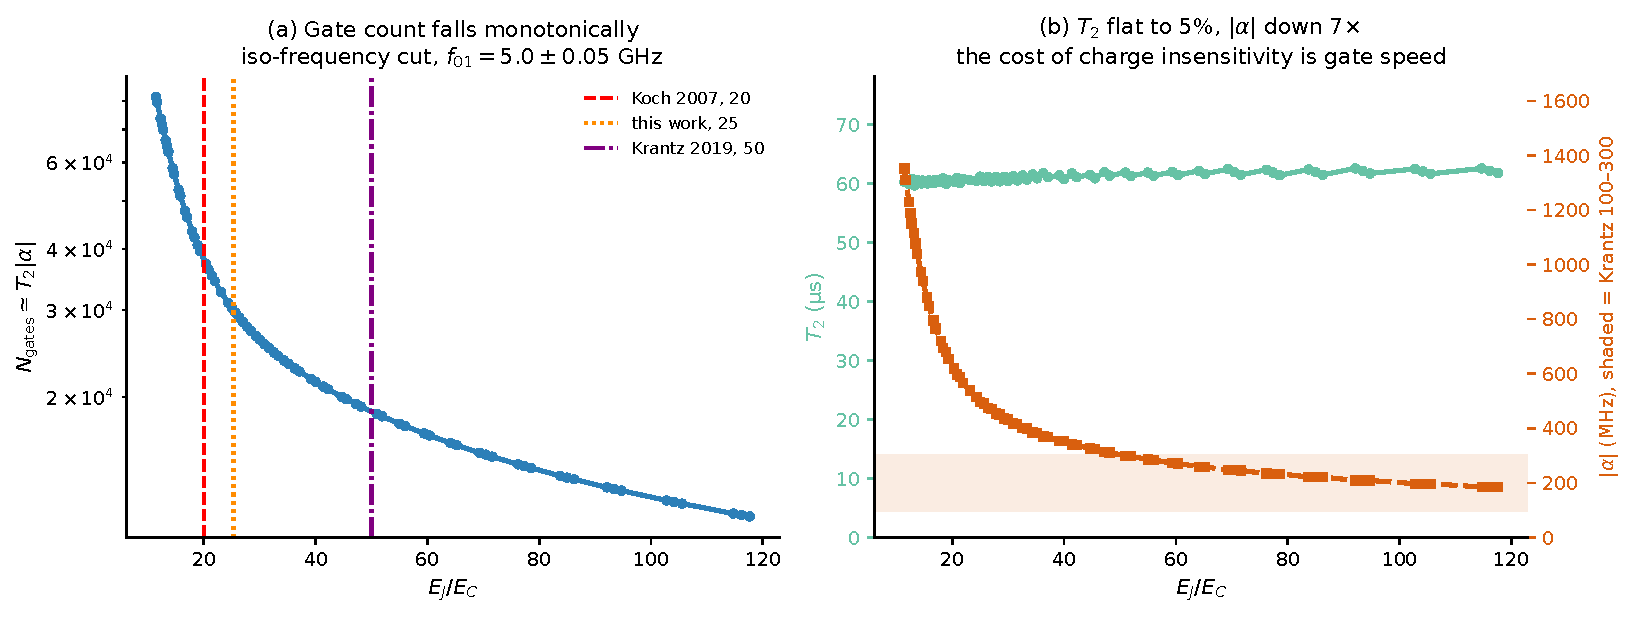
\includegraphics[width=\columnwidth]{figures/transmon_tradeoff.pdf}
\caption{The transmon trade-off at fixed frequency ($f_{01} = 5.00 \pm
\SI{0.05}{\giga\hertz}$). (a) Gate count falls monotonically with $E_J/E_C$; the three
vertical lines are candidate regime thresholds, and the optimum sits on whichever one is
imposed. (b) $T_2$ is flat to 4.8\% while $|\alpha|$ falls $7.3\times$; the shaded band is
the Krantz \SIrange{100}{300}{\mega\hertz} design window. Charge insensitivity costs gate
speed, not coherence.}
\label{fig:tradeoff}
\end{figure}

Holding $f_{01} = 5.00 \pm \SI{0.05}{\giga\hertz}$ and sweeping $E_J/E_C$ from 11.4 to 117.6,
$T_2$ is flat to 4.8\% (\SIrange{59.7}{62.6}{\micro\second}) while $|\alpha|$ falls by a
factor of 7.3 (\SIrange{1353}{185}{\mega\hertz}). \textbf{Charge insensitivity is bought with
anharmonicity---that is, with gate speed---and essentially not with coherence at all}
(Fig.~\ref{fig:tradeoff}).

That the trade is anharmonicity-for-charge-insensitivity is expected from Koch's asymptotics:
with $\alpha \simeq -E_C$ and $f_{01} \simeq \sqrt{8E_JE_C}$ held fixed, raising $E_J/E_C$
forces $E_C \propto (E_J/E_C)^{-1/2}$, predicting a factor 3.21 over our swept range against a
measured $E_C$ ratio of 3.47. The observed $7.3\times$ fall in $|\alpha|$ is steeper still
because $\alpha \simeq -E_C$ is asymptotic and fails at the low end: $|\alpha|/E_C = 2.29$ at
$E_J/E_C = 11.4$ against $1.09$ at $117.6$. The trade-off is therefore harshest exactly in the
low-$E_J/E_C$ corner that an unconstrained gate-count metric wants to select, which is an
independent reason to keep the design envelope.

Relocating the gate-count optimum under eight regime thresholds spanning $E_J/E_C = 15$ to
60, the optimum tracks every one of them to within 0.24. It sits \emph{on} the constraint,
never inside the domain. This is the signature of a constrained optimum, and it means the
substantive choice in this part of the design space is the threshold, not the optimisation. The correct claim is a monotone trade-off terminated wherever the
regime boundary is drawn, and any quoted optimum is meaningful only together with its
threshold. We adopt the Krantz envelope ($E_J/E_C \ge 50$, $|\alpha| \in
[100,300]$\,MHz, $f_{01} \in [3,6]$\,GHz)~\cite{krantz2019} because it is independent of every
noise amplitude in the study, giving the operating point $E_J = \SI{13.0}{\giga\hertz}$,
$E_C = \SI{0.26}{\giga\hertz}$, $f_{01} = \SI{4.92}{\giga\hertz}$,
$T_2 = \SI{62.4}{\micro\second}$, $|\alpha| = \SI{299}{\mega\hertz}$.

A limitation of the model bears on this choice: \texttt{tphi\_1\_over\_f\_ng} covers $1/f$
dephasing only, and the broadband charge sensitivity that motivates Krantz's
$E_J/E_C \ge 50$ is absent. Left to itself the metric under-penalizes low $E_J/E_C$ and would
recommend $|\alpha| \approx \SI{728}{\mega\hertz}$, roughly $2.4\times$ what is fabricated.
The envelope is a constraint imposed on the model, not a result derived from it.

\section{The Fluxonium Design Plane}

Over $E_J \in [3,15]$, $E_L \in [0.2,1.5]$\,GHz at $E_C = \SI{2.5}{\giga\hertz}$ and
$\Phi/\Phi_0 = 1/2$, the same confound appears: $\mathrm{corr}(\log T_2, \log f_{01}) =
-0.9973$. The unconstrained maximum, \SI{5427}{\micro\second}, sits at both grid edges at
$f_{01} = \SI{75}{\mega\hertz}$, where $\bar n_{\rm th} = 3.7$---thermally scrambled and
$2.3\times$ below the lowest published device. Constrained to the published band
\SIrange{0.17}{0.83}{\giga\hertz} the best design gives \SI{2412}{\micro\second} at
$E_J = 11.8$, $E_L = \SI{0.405}{\giga\hertz}$.

\subsection{An interior optimum, created by second-order dephasing}

Extending the scan to $E_J = \SI{45}{\giga\hertz}$ reveals a genuine interior maximum in
$T_2$, present at every $(E_C, E_L)$ combination tested (Fig.~\ref{fig:interior}). It is created by the second-order
flux channel: as $E_J$ rises and $E_L$ falls the qubit sinks into a deep double well,
$f_{01}$ collapses, and $\partial^2 f_{01}/\partial\Phi^2$ grows by three orders of
magnitude across the scan, so $\Gamma_\Phi^{(2)}$ grows with it and eventually overwhelms the
improving dielectric $T_1$. At the turning point that channel carries 43--58\% of the total
dephasing rate, which is the signature of a genuine internal optimum: the channel that turns
the curve over is comparable to everything else exactly at the turn. A first-order-only
pipeline shows no turnover over the same range and rises monotonically to
$2.3\times10^{5}$\,\si{\micro\second}---which is precisely how an earlier version of this
analysis concluded there was no interior optimum, and is a concrete argument for including the
second-order channel in any design study that sweeps toward low $E_L$.

The mechanism is geometric. As $E_J$ rises and $E_L$ falls the potential minima separate, the
tunnel splitting that sets $f_{01}$ collapses, and the same deepening well sharpens the
curvature $\partial^2 f_{01}/\partial\Phi^2$, which grows by three orders of magnitude across
the scan. Since $\Gamma_\Phi^{(2)} \propto \partial^2\omega_{01}/\partial\Phi^2$ by
Eq.~\eqref{eq:secondorder}, second-order dephasing grows with it and eventually overwhelms the
improving dielectric $T_1$. The transmon has no analogue: its charge dispersion falls
exponentially in $\sqrt{E_J/E_C}$ with no turning point.

\begin{figure}[t]
\centering
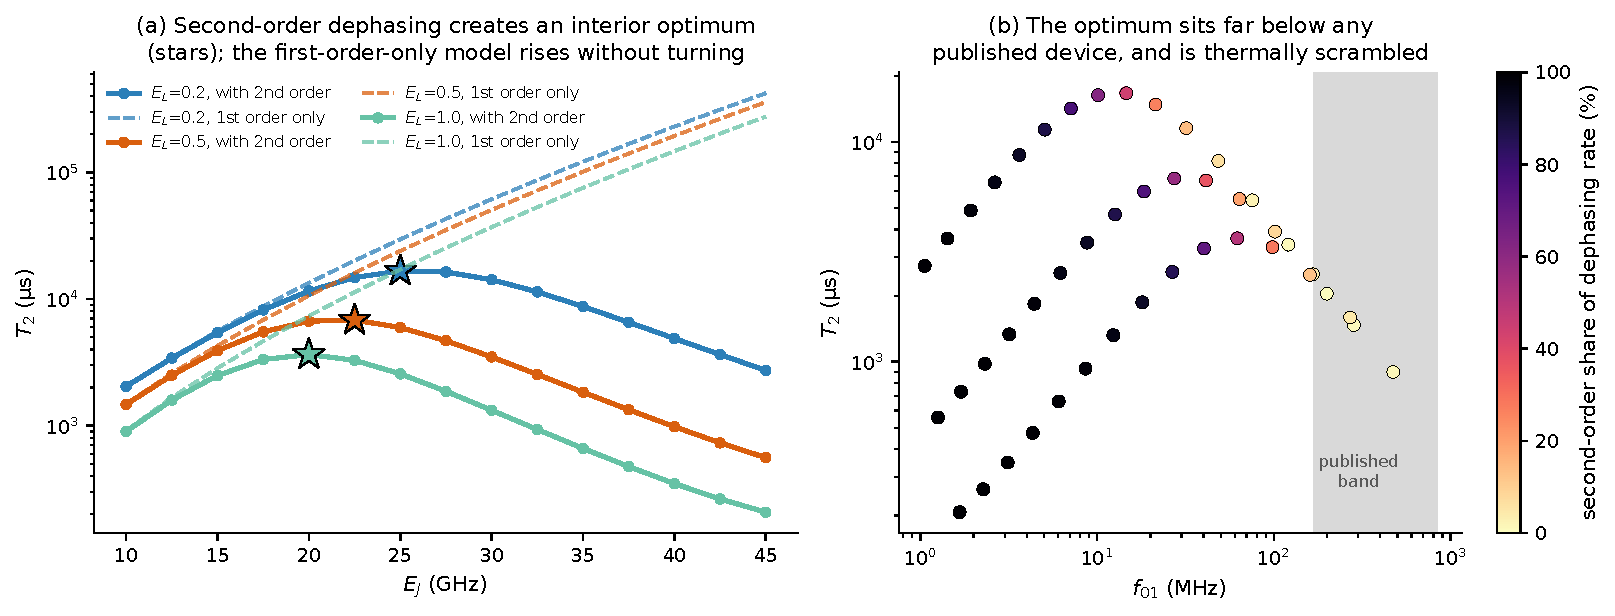
\includegraphics[width=\columnwidth]{figures/fluxonium_interior_optimum.pdf}
\caption{(a) $T_2$ versus $E_J$ at three values of $E_L$. Solid curves include second-order
flux dephasing and turn over (stars); the dashed first-order-only curves rise without limit
over the same range, which is how the interior optimum was previously missed. (b) The same
points against $f_{01}$, coloured by the second-order share of the dephasing rate. Every
turning point lies far below the published fluxonium band (shaded).}
\label{fig:interior}
\end{figure}

The optimum is nevertheless inaccessible. It occurs at $f_{01} = 10$--\SI{75}{\mega\hertz}
with $\bar n_{\rm th} = 4$--32. Past the turnover the frequency correlation reverses sign,
which is a further indication that the second-order channel introduces genuinely new
structure rather than rescaling the old.

\section{Dominant Noise Channels}

At a charge-sensitive bias ($n_g = 0.25$) charge noise dominates the transmon below
$E_J/E_C \approx 25$ and dielectric relaxation above it. That crossover is measured from our
own data and lands close to Koch's independently derived bound of 20; the two arguments are
unrelated---one a noise-budget crossover, the other a pulse-duration requirement---so their
agreement is genuine corroboration. Critical-current noise never dominates anywhere in 1600
points at literature amplitudes. The crossover is noise-model dependent (it spans 20.8--29.9
across literature ranges) and is therefore reported as a result rather than used as an input.

For the fluxonium, relaxation dominates at the sweet spot and first-order flux noise becomes
the largest single term beyond $2.75\times10^{-5}\,\Phi_0$. Quasiparticle tunnelling is not a
dead channel: it is suppressed only \emph{at} the sweet spot, where $f_{01}$ is minimal, and
limits $T_1$ at most detuned points. This finding is conditional on
$x_{qp} = 3\times10^{-6}$, a default that Nguyen \emph{et al.} measure to be $300\times$
lower for their devices; at their density the channel is negligible everywhere. It is the
most fragile result in the study and is reported as conditional.

\section{The Cross-Architecture Comparison}

\subsection{Bias robustness, the one unambiguous asymmetry}

Both bias coordinates are periodic with period one, so the width of the window over which
$T_2$ stays within a factor $k$ of its sweet-spot value, as a fraction of one bias period, is
directly comparable. The transmon's $T_2$ varies by $1.0056\times$ across its \emph{entire}
charge period---a factor-of-two loss never occurs at any bias. The fluxonium loses a factor
of two within $\pm 3.61\times10^{-5}\,\Phi_0$ and a factor of ten within
$3.25\times10^{-4}\,\Phi_0$, located by root-finding on the model rather than read off a
grid. The usable bias window differs by $1.4\times10^{4}$.

The falloff exponent is not a single number. It approaches the first-order $1/f$ prediction
of $-1$ only in an intermediate window where $T_2$ is genuinely flux-dephasing limited,
reaching $-0.956$ there, and flattens on both sides---capped by the $2T_1$ ceiling close in,
and contaminated by other channels far out.

Intrinsic $1/f$ flux noise does not by itself drive the qubit off the spot: even at Nguyen's
measured amplitude integrated over an hour, the RMS wander leaves a $24\times$ margin to the
tenfold-loss detuning. The binding constraint is systematic drift and bias-line calibration,
not stochastic noise---which relocates the difficulty rather than removing it, and makes it
scale with qubit count.

\textbf{This constraint is being engineered away, which we should say plainly.} B\'en\^atre
\emph{et al.} hold gradiometric fluxonium qubits at their sweet spot passively, reporting
stability of $3\times10^{-4}\,\Phi_0$ from target with only a 15\% reduction in echo
coherence~\cite{benatre2025}. Their achieved stability sits essentially at our computed
tenfold-loss detuning of $3.25\times10^{-4}\,\Phi_0$, yet they observe far less degradation
than that number would suggest---unsurprisingly, since their device has different $E_L$ and
hence different curvature, and echo suppresses low-frequency drift that free induction does
not. We read their result as evidence that the bias-precision cost we quantify is real,
understood, and addressable by design rather than by calibration alone. It weakens the
scalability pessimism in our conclusion without touching the arithmetic behind it.

\subsection{No single ratio}

Table~\ref{tab:q3} gives the comparison under every metric we consider defensible, and
Fig.~\ref{fig:robust} shows how each fares across the noise band.

\begin{table}[t]
\caption{Fluxonium/transmon ratio by metric. MC = median over $N=400$ log-uniform draws of
each noise amplitude across its literature decade, with the 5--95\% sample spread.}
\label{tab:q3}
\centering
\small
\small
\setlength{\tabcolsep}{4pt}
\begin{tabular}{@{}lccc@{}}
\toprule
Metric & Det. & MC med.\ [5--95\%] & Wins\\
\midrule
Raw $T_2$                       & $18.1$      & $11.3$ [3.6, 21.1]   & 100\%\\
$T_2$, matched $f_{01}$         & $1.1$--$2.2$ & $\mathbf{0.86}$ [0.27, 1.6] & \textbf{42\%}\\
Gates, $1/|\alpha|$             & $524$       & $326$ [104, 611]     & 100\%\\
Gates, $1/\min(|\alpha|,f_{01})$ & $22.0$     & $13.7$ [4.4, 25.6]   & 100\%\\
Gates, $1/f_{01}$               & $\mathbf{1.34}$ & $\mathbf{0.83}$ [0.26, 1.6] & \textbf{40\%}\\
Gates, simulated                & $48$        & --                   & --\\
\midrule
Bias window, $2\times$ loss     & \multicolumn{3}{c}{$1.4\times10^{4}$ wider for the transmon}\\
\bottomrule
\end{tabular}
\end{table}

Two ranges are visible, and they are of comparable size. \emph{Across} metrics the answer
spans roughly $700\times$. \emph{Within} the gate-count metric alone it spans $393\times$,
depending on what bounds the minimum pulse length. The $|\alpha|$ bound---leakage to
$|2\rangle$ only---is the textbook choice, but for a fluxonium at half flux
$|\alpha| = \SI{8.7}{\giga\hertz}$ is $24\times$ the transition frequency it would drive, so
that bound licenses a pulse $24\times$ shorter than one period of the transition itself. The
drive-period bound $1/f_{01}$ is equally physical and gives $1.34\times$.

\begin{figure}[t]
\centering
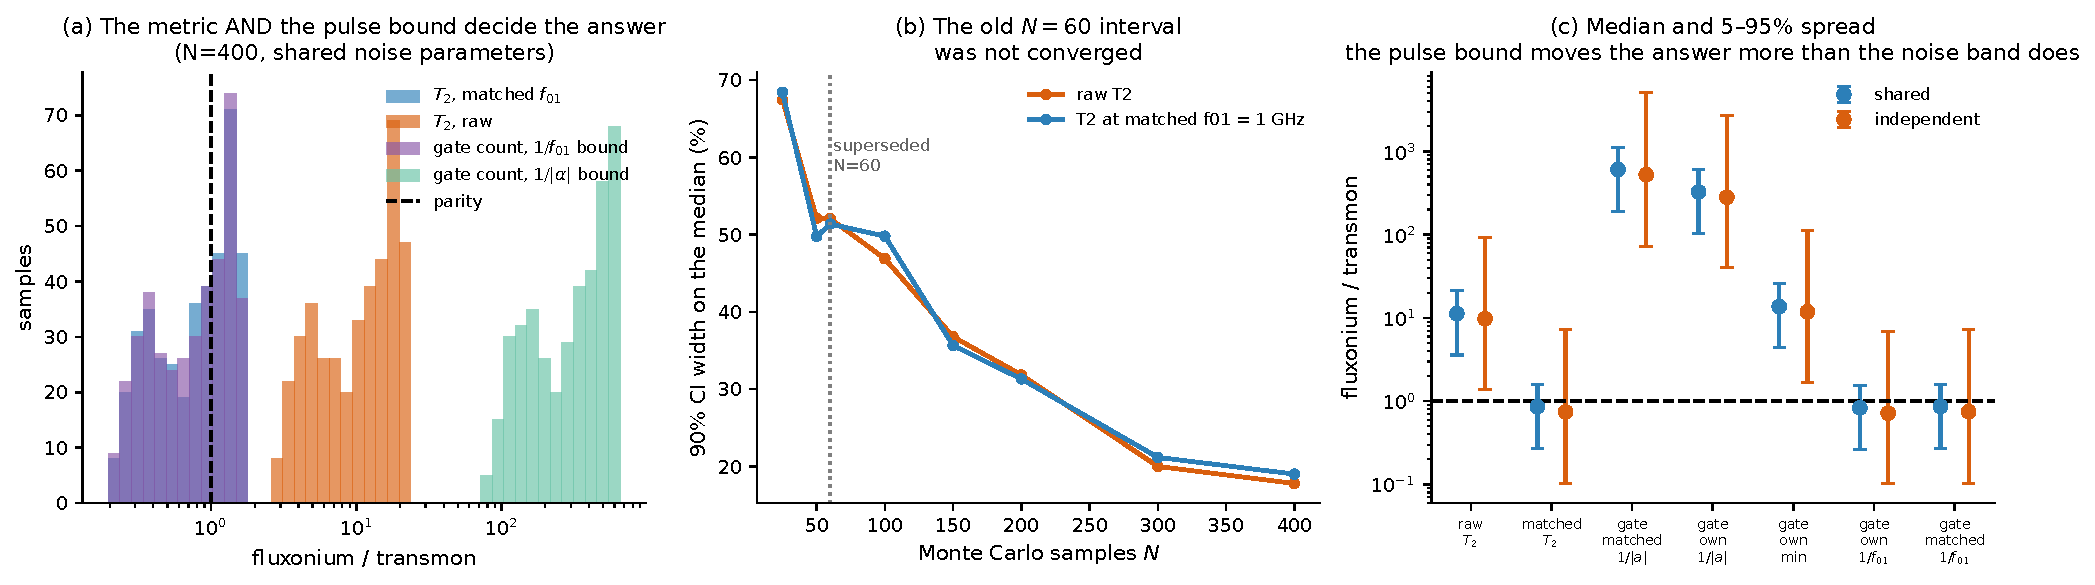
\includegraphics[width=\columnwidth]{figures/q3_robustness.pdf}
\caption{Robustness of the Q3 answer to the noise amplitudes. (a) Distribution of the
fluxonium/transmon ratio under four metrics, $N=400$ shared-parameter draws; the metric and
the pulse bound each move the answer by more than the noise band does. (b) The 90\%
bootstrap CI on the median against sample size, showing that an earlier $N=60$ interval had
not converged. (c) Median and 5--95\% spread per metric under shared versus independent
sampling.}
\label{fig:robust}
\end{figure}

\subsection{The raw advantage is mostly frequency}

The two devices differ in frequency by $13.6\times$, and
$\log 13.55/\log 18.10 = 0.90$: about 90\% of the log-advantage is the frequency difference.
This is not a coincidence of these two designs. Dielectric loss dominates both architectures
and its rate scales with $\omega_{01}$, so $T_2 \propto 1/f_{01}$ in both---measured as
$f_{01}^{-0.965}$ for the transmon. Because the flux sweet spot \emph{is} a frequency
minimum, the fluxonium is structurally advantaged on any uncontrolled $T_2$ comparison, and
reporting one credits the architecture with what the frequency did.

Controlling for it, the deterministic ratio at matched $f_{01}$ is 1.07--2.16$\times$. But
propagated across the literature noise band the median is $0.86\times$ and the fluxonium wins
in only 42\% of samples. \textbf{At matched frequency the transmon is more often the better
device.} This is the most important negative result here: what remains of the coherence
advantage after the frequency control does not survive the noise-amplitude uncertainty.

\subsection{Settling the pulse bound}
\label{sec:pulse}

The gate-count range is wide enough to make the metric almost uninformative, so we settle it
by simulation rather than by argument. We integrate the lab-frame Schr\"odinger equation for
each architecture with no rotating-wave approximation, using a six-level truncation of the
\texttt{scqubits} eigenbasis and a charge drive, and calibrate each gate as an experimentalist
would: amplitude, DRAG coefficient~\cite{motzoi2009} and Stark-shifted drive frequency are
optimized at every duration, and the average gate error is evaluated on the computational
subspace so that leakage is counted; Fig.~\ref{fig:pulse} shows the resulting error curves.

This exposes an effect that the anharmonicity argument misses entirely. The fluxonium's
$|\alpha|/f_{01} = 24$ looks decisive, but its drive matrix elements are unfavourable: at
half flux $|\langle 1|\hat n|2\rangle| / |\langle 0|\hat n|1\rangle| = 10.2$, against $1.37$
for the transmon. The drive couples ten times more strongly to the leakage transition than to
the qubit transition, so the effective figure of merit is the anharmonicity divided by that
ratio, not the anharmonicity itself.

Table~\ref{tab:pulse} reports the shortest calibrated gate reaching an average error below
$10^{-3}$ for each architecture, and the resulting gate count. \emph{These durations are upper
bounds}: a three-parameter calibration over a fixed Gaussian shape is far from optimal
control, and GRAPE or CRAB over a free pulse shape would shorten both---not necessarily
equally. The point is not the precise value but that the simulated ratio falls decisively
between the two naive bounds, excluding both.

\begin{table}[t]
\caption{Shortest calibrated $X$ gate reaching an average error below $10^{-3}$, from the
lab-frame simulation, and the resulting gate count $N = T_2/T_{\rm gate}$. Durations are
upper bounds and are bracketed by the duration grid and by optimiser convergence.}
\label{tab:pulse}
\centering
\begin{tabular}{lccc}
\toprule
 & $T_{\rm gate}$ (ns) & $T_2$ (\si{\micro\second}) & $N$\\
\midrule
Transmon  & $8.0$ ($6.0$--$8.0$)  & $62.4$   & $7{,}803$\\
Fluxonium & $3.0$ ($2.5$--$3.0$) & $1129.7$ & $376{,}571$\\
\midrule
\multicolumn{3}{l}{\textbf{Simulated ratio}} & $\mathbf{48\times}$\\
\multicolumn{3}{l}{\quad bracket from grid + optimiser} & $36$--$58\times$\\
\multicolumn{3}{l}{\quad for comparison, $1/|\alpha|$ bound} & $524\times$\\
\multicolumn{3}{l}{\quad for comparison, $1/f_{01}$ bound} & $1.34\times$\\
\bottomrule
\end{tabular}
\end{table}

The result is that the fluxonium does convert coherence into operations more efficiently than
the transmon, but by a factor of order $36$--$58\times$ rather than the ${\sim}500\times$ the anharmonicity bound suggests or the ${\sim}1\times$ the drive-period bound suggests. Neither extreme survives contact with a simulated pulse, and the residual uncertainty is dominated by optimiser convergence rather than by physics.

\begin{figure}[t]
\centering
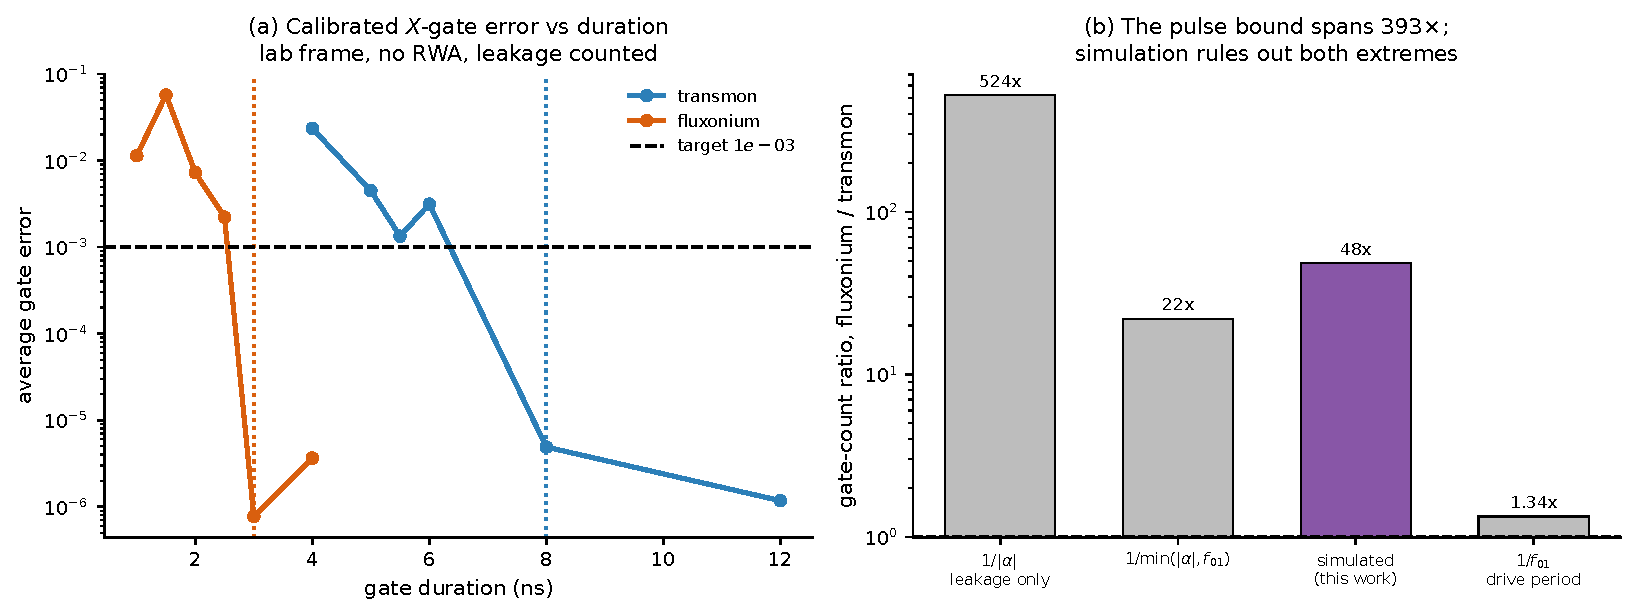
\includegraphics[width=\columnwidth]{figures/q3_pulse_bound.pdf}
\caption{(a) Average $X$-gate error against gate duration for both architectures, from the
lab-frame simulation with amplitude, DRAG and Stark detuning calibrated at each point;
dotted lines mark the shortest duration meeting the $10^{-3}$ target. Non-monotonicity at the
shortest durations is optimiser noise and is not smoothed. (b) The gate-count ratio under
each pulse-length bound. The two analytic bounds differ by $393\times$; the simulation
(purple) falls between them and excludes both.}
\label{fig:pulse}
\end{figure}

\section{Calibration Against Measurement}
\label{sec:calibration}

Run at the parameters of each of the nine devices in the published Table~I of Nguyen
\emph{et al.}, the model is optimistic by a median factor of $2.0\times$ on $T_1$ and
$2.6\times$ on $T_2$, worst case $5.7\times$. The gap is not uniform, so it is not a single
missing constant---and it is smallest where it matters most: device~I, the device nearest our
nominal design in frequency (0.395 versus \SI{0.363}{\giga\hertz}), is matched to 4\% on
$T_2$, with the model \emph{pessimistic} on its $T_1$.

Identified contributors, in order: the flat $Q_{\rm cap} = 10^6$ against their measured
$\tan\delta_C = (2.0$--$3.6)\times10^{-6}$ at \SI{6}{\giga\hertz}; the absence of Purcell
decay, photon shot noise and inductive loss; the fact that their $T_2$ is a Hahn echo while
this model computes free-induction decay, which makes the comparison conservative in the
model's favour; and a temperature mismatch, since we run at the \SI{15}{\milli\kelvin}
default while they state \SI{20}{\milli\kelvin}.

The comparison also has a floor set by our own model rather than by the devices. Absolute
$T_2$ spans \SIrange{149}{3316}{\micro\second} under single-decade moves of the noise
amplitudes, so a factor of $2.6$ is well inside the band the model itself admits; the
calibration should be read as establishing the right order of magnitude, not as a residual to
be explained away. Consistent with that, the state of the art has moved well past the devices
we calibrate against---Somoroff \emph{et al.} report $T_2 = 1.43$\,ms~\cite{somoroff2023}, so
a model tuned to reproduce Nguyen's 2019 numbers exactly would now be miscalibrated against
2023 hardware.

We stress that the published table must be used. The arXiv v1 preprint lists eight devices
and omits device~I entirely---the paper's headline device, and the one closest to the design
regime studied here.

\section{Limitations}

The model omits Purcell decay, photon shot noise, inductive loss in the junction array, TLS
spectral structure, crosstalk and any lattice; qubits are treated in isolation. The
superinductance is ideal, so array-mode hybridization is absent, though
Section~\ref{sec:validation} bounds that omission at $-0.43\%$ in $f_{01}$ at the flux sweet
spot. Second-order dephasing uses a convention with no logarithmic factor; a $\ln^2$
convention would change sweet-spot $T_2$ by ${\sim}37\%$ instead of 0.6\% and would move,
though not remove, the interior optimum. Absolute $T_2$ spans
\SIrange{149}{3316}{\micro\second} under single-decade moves of the noise amplitudes and
should never be quoted without a band. The Monte Carlo varies amplitudes only; fabrication
spread in $E_J$, $E_C$, $E_L$ is not propagated, and the log-uniform priors are a choice. The
gate-count metric is a heuristic, not a literature formula.

\section{Conclusion}

Neither architecture has a coherence sweet spot in design space. Both design planes are, to
better than $|r| = 0.99$, restatements of the transition frequency, so a raw $T_2$ maximum
locates the edge of the swept domain or the point where a frequency constraint was drawn.
The transmon is a monotone trade-off in which charge insensitivity is paid for in
anharmonicity, once, at design time. The fluxonium has a real interior optimum, visible only
once second-order flux dephasing is included, but it is thermally out of reach; in practice
it too is a trade-off terminated by a frequency floor.

For Q3, the honest output is a metric family, not a number. The fluxonium's raw $18\times$
coherence advantage is roughly 90\% frequency; at matched frequency it inverts to a median
$0.86\times$ across the literature noise band. Its durable advantage is anharmonicity per
unit coherence, and its price is operating-point precision---a bias window four orders of
magnitude narrower than the transmon's, paid continuously at run time rather than once at
design time. Whether that trade is worth making is a question about qubit count and
calibration budget, not about coherence.

More generally, we suggest that architecture comparisons in this field should state the
metric, the control variable and the uncertainty band together. A single ratio between two
architectures at their own operating points is not a comparison between architectures.

\section{Outlook}

Two extensions would sharpen the results most. The gate-count metric is currently settled by a
coarse calibration; optimal control over a free pulse shape (GRAPE or CRAB) would tighten the
$36$--$58\times$ bracket and, more interestingly, would test whether the fluxonium's
unfavourable leakage matrix element can be shaped around---the anharmonicity is genuinely
there, and a pulse that exploits it without driving $|1\rangle \to |2\rangle$ would move the
number back toward the leakage-only bound. Second, the interior fluxonium optimum we find is
thermally inaccessible at \SI{15}{\milli\kelvin}, but that is a statement about temperature as
much as about design; the same analysis at lower base temperature, or with active
initialisation modelled, would establish whether it is inaccessible in principle or merely
inconvenient.

A broader point follows from the metric sensitivity. If a single architecture comparison can
span two orders of magnitude depending on choices that are all defensible, then comparisons
reported as single ratios carry less information than they appear to. We would encourage the
practice McRae \emph{et al.}~\cite{mcrae2021} advocate for experimental coherence
numbers---report the conditions with the number---to be extended to modelled design
comparisons: state the control variable, state the figure of merit, and give the spread.

\section*{Acknowledgements}

The interpretation sections of the underlying notebooks, and the first draft of this
manuscript, were prepared with the assistance of a large language model (Claude, Anthropic)
working from the committed numerical artifacts. All physics, numerical results and final
claims are the author's responsibility. This disclosure is made in line with IEEE policy on
the use of artificial intelligence in authorship.

\section*{Reproducibility and Data Availability}

All code, generated data and figures are openly available at
\url{https://github.com/ishitabera/quantum-coherence-sweet-spots-transmon-fluxonium}.

Every number in this paper is produced by five notebooks run in order from a single validated
pipeline; no notebook reimplements the physics. Each sweep writes its raw data before any
figure code executes, together with a metadata record of the grid, the noise amplitudes, the
software versions and the git revision. Every quoted value is bound to the file and filter
that produced it by an automated provenance ledger of 32 entries, which recomputes and asserts
each one on every run and fails rather than warns if a value drifts from its artifact. A test
suite of 32 checks pins the conventions and the validated anchors, including the published
numbers used for calibration.

\bibliographystyle{IEEEtran}
\bibliography{refs}

\end{document}
